\documentclass[../main]{subfiles} 

% \title{Integration 1}
% \date{November 13 to 17.}

% {Stewart (9E). Section 4.9 (pages 356 to 364), Appendix E (pages A36 to A41), and Section 5.1 (pages 372 to 384). }

\begin{document}


%--------------------------------------------------
%
% instructor notes
%
%--------------------------------------------------
Notes.
  \begin{itemize}
    \item Students should bring scissors to lectures this week.  Please exercise safety precautions when using scissors.
  \end{itemize}




%--------------------------------------------------
%
% learning objectives
%
%--------------------------------------------------

  At the end of the lecture, students should be able to
  \begin{itemize}
    \item recognize antiderivatives of functions and use antiderivatives to solve real-world problems,
    \item evaluate and manipulate summations expressed using \(\sum\) (the Sigma notation),
    \item use rectangles to approximate areas under a curve \(y = f(x)\), 
    \item understand geometric interpretation of the definition of the area under a curve \(y = f(x)\), and
    \item express the distance problem as an area under the curve problem.
  \end{itemize}




%--------------------------------------------------
%
% General instructions
%
%--------------------------------------------------
% \begin{instruction}[Instruction]{How to ...}
%   \begin{enumerate}[label=(\alph*)]
%     \item TODO
%   \end{enumerate}
% \end{instruction}
%



%--------------------------------------------------
%
% activities
%
%--------------------------------------------------
\begin{outline}{sec}{Antiderivatives}{page} \label{outline:antiderivatives}
  \begin{enumerate}
    \item A rock at rest is launched straight up with initial velocity \(v_{0}\) metres per second. The object's vertical velocity function with respect to time \(t\) is
      \begin{equation} \label{eq:rock}
        v(t) = v_{0} - g t, 
      \end{equation}
      where \(g\) is the acceleration due to gravity (approximately 9.8 \(m/s^{2}\)). Discuss possible height functions of the rock assuming \emph{all} measurements are taken \emph{from the sea level}.

    \item \textbf{Definition}.
      \begin{mdframed}[style=simple]
        Let \(f\) be a function. A function \(F\) is called an \emph{antiderivative} of \(f\) on an interval \(I\) if 
        \[ F'(x) = f(x) \text{ for all } x \text{ in } I. \]
      \end{mdframed}

      Note if an antiderivative exists for a function \(f\), then \(f\) has infinitely many antiderivatives. 

    \item \textbf{Theorem}.
      \begin{mdframed}[style=simple]
        Let \(f\) be a function. If \(F\) is an antiderivative of \(f\) on an interval \(I\), then \emph{the most general} antiderivative of \(f\) on \(I\) is \(F(x) + C\) where \(C\) is an arbitrary constant.
      \end{mdframed}

      Remark that this statement is both a theorem and a definition. See Table~\ref{table:antiderivatives} for a list of commonly used antiderivatives.
      \begin{table}[h]
        \centering
        \includegraphics{../standalones/build/table_antiderivatives}
        \caption{A list of common antiderivatives.\\Filing in the third column is an additional exercise.}
        \label{table:antiderivatives}
      \end{table}

    \item Find the most general antiderivative of the functions \(f(x) = \cos(x)\) and \(g(x) = x^{n}\). Discuss possible cases for \(n\). \faIcon{comment} Can you apply the above formula when \(n\) is \emph{not} an integer?

    \item Discuss what functions are their own antiderivatives. \faIcon{comment} Is the constant function \(f(x) = 1\) its own antiderivative?

    \item Find the function \(f\) if \(f'(x) = \sin(x) + e^{x} - \frac{1}{x}\) and \(f(1) = 3\).
    \item The linear density of a rod of length \(1\) metre is given by \(\rho(x) = \frac{1}{\sqrt{x}}\), in grams per centimetre, where \(x\) is measured in centimetres from one end of the rod. Find the mass of the rod. % Stewart Problem 78.
    \item {Antiderivative\emph{s} of a function \(f(x)\) are a \emph{family} of functions whose derivatives are all equal to \(f(x)\). If \(F(x)\) is a particular antiderivative of \(f(x)\), then \(F(x) + C\) where \(C\) stands for a constant is the most general antiderivative of \(f(x)\). }
    \item {It is always possible to check if you have found a antiderivative. To see if a function \(F(x)\) is an antiderivative of a function \(f(x)\), check whether \(F'(x) = f(x)\) is true.}
  \end{enumerate}
\end{outline}



\begin{outline}{sec}{Sigma notation of summation}{page} \label{outline:summation}
  \begin{enumerate}
    \item The Greek letter \(\Sigma\) (capital sigma) is used to express summations in a succinct way. Let \(a_{m}, a_{m+1}, \dots, a_{n}\) be numbers where \(m,n\) are integers such that \(m \le n\).  We define
      \begin{mdframed}[style=simple]
        \[ \sum_{i=m}^{n} a_{i} = a_{m} + a_{m+1} + \cdots + a_{n}, \text{ if } m \le n. \]
      \end{mdframed}
      The integer \(i\) is called the \emph{index of summation}. Some literature refers to \(i\) as the dummy variable.

    \item \textbf{Theorem}. Suppose \(c\) is a constant. Then
      \begin{mdframed}[style=simple]
        \begin{enumerate}[label=(\alph*)]
          \item \(\sum_{i=m}^{n} c \, a_{i} = c \sum_{i=m}^{n} a_{i}\).
          \item \(\sum_{i=m}^{n} (a_{i} + b_{i}) = \sum_{i=m}^{n} a_{i} + \sum_{i=m}^{n} b_{i}\).
          \item \(\sum_{i=m}^{n} (a_{i} - b_{i}) = \sum_{i=m}^{n} a_{i} - \sum_{i=m}^{n} b_{i}\).
        \end{enumerate}
      \end{mdframed}

    \item A list of rectangles \(R_{-3/2}, R_{-1}, R_{-1/2}, R_{0}, R_{1/2}, R_{1}, R_{3/2}, R_{2}, R_{5/2}\) all have width \(\frac{1}{2}\). The rectangle \(R_{\alpha}\) has height \(\alpha^{2}\). See Figure~\ref{fig:rectangles}. 
      \begin{enumerate}
        \item Express the areas of the rectangles as a list of numbers. Choose appropriate \emph{integers} for the subscripts. 
        \item Express the \emph{sum of their areas} using the sigma notation.
      \end{enumerate}
      \begin{figure}[h]  % [h] for here, [ht] for here top, [hb] for here bottom
        \centering
        \includegraphics[height=2.5in]{../standalones/build/plot_rectangles}
        \caption{Express the sum of areas of shaded rectangles using the sigma notation.\\Notice the rectangles are purposely stretched wider to fit the labels on top.}
        \label{fig:rectangles}
      \end{figure}

    \item Use the formula \(\sum_{i=1}^{n} i = \frac{n(n+1)}{2}\) to simplify \(\sum_{i=3}^{n} (2i+1)\). For an explanation of the formula \(\sum_{i=1}^{n} i = \frac{n(n+1)}{2}\), see the end of the document.

    \item Use the formula \(\sum_{i=1}^{n} i^{2} = \frac{n(n+1)(2n+1)}{6}\) to evaluate the limit \(\lim_{n \to \infty} \sum_{i=1}^{n} \frac{1}{n} \left( \frac{i}{n} \right)^{2}\). % Stewart (9E), exercise 43 in Appendix E.

      % \begin{itemize}
      %   \item[\faIcon{comment}] Can you interpret the sum \(\sum_{i=1}^{n} \frac{1}{n} \left( \frac{i}{n} \right)^{2}\) geometrically given \(n = 4\)? 
      %
      %     One method is to find \(n\) rectangle of \emph{equal width} such the sum of their areas is the given sum. 
      %
      %   \item[\faIcon{comment}] What if \(n = 5,6,7\)? What happens when \(n\) goes to infinity?
      % \end{itemize}

    \item {The Sigma notation is a succinct way to express the addition of some numbers.}
  \end{enumerate}
\end{outline}



\begin{outline}{sec}{The Area Problem}{page} \label{outline:area}
  \begin{enumerate}
    \item (Group activity) 
      \begin{enumerate}
        \item Invent a method of approximation to estimate the area of some farms in Richmond, BC, as shown in Figure~\ref{fig:integral_farms}. For simplicity, assume houses are included. Can you write down a formula using the sigma notation for your approximation?
          \begin{figure}[h]  % [h] for here, [ht] for here top, [hb] for here bottom
            \centering
            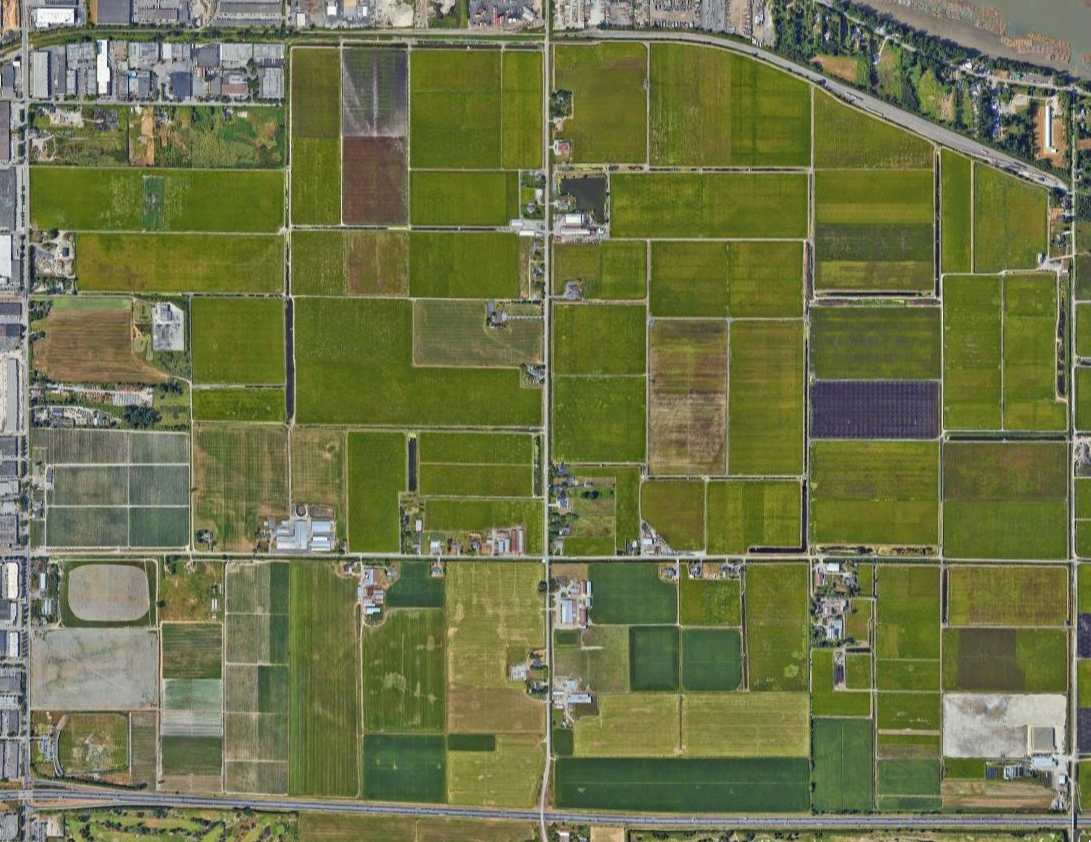
\includegraphics[height=2in]{../standalones/photo_farms}
            \caption{How can we approximate the area of these farms? Hint: Use scissors!}
            \label{fig:integral_farms}
          \end{figure}

        \item Use your method of approximation to estimate the area of York University's Keele campus as shown in Figure~\ref{fig:integral_campus}. Can you write down a formula using the sigma notation for your approximation?
          \begin{figure}[h]  % [h] for here, [ht] for here top, [hb] for here bottom
            \centering
            \includegraphics[height=2in]{../standalones/photo_campus}
            \caption{How can we approximate the area of York University's Keele campus? Hint: Use scissors!}
            \label{fig:integral_campus}
          \end{figure}

        \item[\faIcon{star}] Generalize and refine students' methods of approximation towards Equation~\eqref{eq:area}.
      \end{enumerate}

    \item {The \emph{area} \(A\) of the region \(S\) that lies under the graph of a \emph{continuous} function \(f\) is the limit of the sum of the areas of approximating rectangles}
        \begin{mdframed}[style=simple]
          \begin{equation} \label{eq:area}
            A = \lim_{n \to \infty} \left[ f(x_{1}) \Delta x + f(x_{2}) \Delta x + \cdots + f(x_{n}) \Delta x \right].
          \end{equation}
        \end{mdframed}
        This definition appears as ``\textcolor{orange}{\fbox{2} Definition}'' in Section 5.1 (page 377) of the textbook. This definition contains several implicit statements.
      \begin{enumerate}
        \item It is implicit that the region \(S\) is the region that lies above the horizontal axis, below the curve \(y = f(x)\), to the right of some vertical line \(x = a\), and to the left of some vertical line \(b\). 
        \item It is implicit that the curve \(y = f(x)\) does not go below, but is allowed to touch, the horizontal axis over the interval \([a,b]\). % \textit{Instructor only: See the definition \(S = \{ (x,y) : a \le x \le b, 0 \le y \le f(x) \}\) inside the box of Figure~1 (page 372) of the textbook.}
        \item The symbol \(n\) represents the number of approximating rectangles. % and only takes values in positive integers. However, one can ignore this information when applying limit laws.
        \item The symbol \(\Delta x\) depends on the integer \(n\) and is defined as \(\Delta x = \frac{b-a}{n}\). 
        \item The numbers \(x_{1}, x_{2}, \dots, x_{n}\) are given by \(x_{i} = a + i \Delta x\) for \(i = 1, \dots, n\). They are the \emph{right} endpoints of the subintervals of \([a,b]\) defined by the approximating rectangles.
      \end{enumerate}

    \item Relate Equation~\eqref{eq:area} to the activity labelled \faIcon{star}.
    \item Show the area under the curve \(y = x^{2}\) from \(a = 0\) to \(b = 1\) approaches \(\frac{1}{3}\).
    \item Discuss examples of computing areas under the curve.

    \item {Let \(f(x)\) be a \emph{continuous} function whose curve \(y = f(x)\) never goes below the horizontal axis. The area below the curve \(y = f(x)\) from \(x=a\) to \(x=b\) where \(a < b\) can be approximated using rectangles. The area below the curve is \emph{defined} to be the expression in Equation~\eqref{eq:area}.}
    \item {The restriction that the curve \(y = f(x)\) must appear above the horizontal axis will be loosened in a future lecture. We will introduce a more general concept called ``net area.''}
  \end{enumerate}

\end{outline}



\begin{outline}{sec}{The Distance Problem}{page} \label{outline:distance}
  \begin{enumerate}
    \item The distance of an object travelling in a straight line at a \emph{constant} velocity can be computed by
      \[
        \text{distance} = (\text{constant velocity}) \times \text{time}.
      \]

    \item Consider the rock example in Outline~\ref{outline:antiderivatives} whose function is given in Equation~\eqref{eq:rock}. Assume the initial velocity \(v_{0}\) is \(2\) metres per second. Let \(h(t)\) be the height function, measured from the sea level, from the time at launch to some time \(t\). Assume we are 200 metres above the sea level.
      \begin{enumerate}
        \item Express the problem of finding \(h(t)\) as an area under the curve problem.
        \item Approximate \(h(1)\) from \(v(t)\) by subdividing the interval \([0,1]\) into \(5\) equal-width rectangles.
      \end{enumerate}

    \item Discuss the interpretation of the area below the curve on Figure~\ref{fig:rock}. 
      \begin{figure}[h!]  % [h] for here, [ht] for here top, [hb] for here bottom
        \centering
        \includegraphics[width=2in]{../standalones/build/plot_rock}
        \caption{A plot of the function in Equation~\eqref{eq:rock} where \(v_{0} = 2\;m/s\).}
        \label{fig:rock}
      \end{figure}
  \end{enumerate}
\end{outline}



%--------------------------------------------------
%
% additional problems
%
%--------------------------------------------------
Exercises.
\begin{enumerate}
\item Find antiderivatives of \(\frac{e^{x} - e^{-x}}{2}\) and \(\frac{e^{x} + e^{-x}}{2}\).
\item Fill in the third column of Table~\ref{table:antiderivatives}.
\item What is an antiderivative of \(\frac{1}{x}\) if \(x < 0\)? You should get an expression without the absolute value sign.
\item What is an antiderivative of \(\frac{1}{x}\) if \(x > 0\)? You should get an expression without the absolute value sign.
\item Is it true that
  \[
    \left( \sum_{i=m}^{n} a_{i} \right) \left( \sum_{i=m}^{n} b_{i} \right) = \sum_{i=1}^{n} a_{i} b_{i}
    \quad\text{and}\quad
    \dfrac{\sum_{i=m}^{n} a_{i}}{\sum_{i=m}^{n} b_{i}} = \sum_{i=m}^{n} \frac{a_{i}}{b_{i}}
  \]
  for an arbitrary list of numbers \(a_{m}, a_{m+1}, \dots, a_{n}, b_{m}, b_{m+1}, \dots, b_{n}\)? If not, find a list of numbers \(a_{1}, a_{2}, b_{1}, b_{2}\) such that these two formulas do not hold.
  \item From the textbook, exercises  1-24, 29-49, 55-61, 65-72, 78, 83 in Section 4.9%Avoiding sinh, cosh
  \item From the textbook, True-False Quiz (questions 1-21) on page 364 to 365; there are also questions that review
Chapter 4 on pages 365 to 368.
    \item From the textbook, exercises 1-36, 43-45, 47 in Appendix E%Avoid telescoping sums
    \item  From the textbook, exercises   1-5, 13-14, 16-18, 20-25  in Section 5.1%avoid upper and lower sums
\end{enumerate}



\noindent\textbf{Appendix}. For every integer \(n \ge 1\), we have a formula
\begin{equation} \label{eq:sums_of_i}
  \sum_{i=1}^{n} i = \frac{n(n+1)}{2}
\end{equation}
      
Figure~\ref{fig:sums_of_i} demonstrates why the formula works in the case \(n=5\). In general, we place \(1\) pink box in the leftmost column, \(2\) pink boxes in the second leftmost column, and so on. The number of pink boxes is \(\sum_{i=1}^{n} i\) which is the left-hand side of Equation~\eqref{eq:sums_of_i}. The index \(i\) in the summation correspond to the \(i\)th leftmost column. Now we place \(n\) blue boxes on top of the pink box in the leftmost column, \(n-1\) blue boxes on top of the pink boxes in the second leftmost column, and so on. Then in each column, the total number of boxes, regardless of the colour, are always \(n+1\). There are \(n\) columns and in each column there are \(n+1\) boxes, regardless of the colour. So the total number of boxes is \(n(n+1)\). We placed the boxes so that there are exactly the same number of pink boxes and blue boxes. We can conclude that the number of pink boxes expressed as \(\sum_{i=1}^{n} i\) is exactly \(\frac{n(n+1)}{2}\).

\begin{figure}[h]
  \centering
  \includegraphics[height=1in]{../standalones/build/proof_sums_of_i}
  \caption{A pictorial explanation of \(\sum_{i=1}^{n} i =  \frac{n(n+1)}{2}\) when \(n = 5\).}
  \label{fig:sums_of_i}
\end{figure}

\end{document}
